\section{A UTxO Model}\label{sec:utxo_model}

We abstract a distributed ledger as a state machine on which parties act.
Specifically, we consider only \emph{payments}, \ie value transfers of
\emph{fungible} assets between parties.

Initially, we assume a ledger state $\ledgerState_{init}$, on which a
\emph{transaction} is applied to move the ledger to a new state. Transactions
that may be applied on a state are \emph{valid}, following a validation
predicate. Each transaction is unique and moves the system to a unique state;
with hindsight, we assume that the ledger never transitions to the same state
(cf. Definition~\ref{def:lstate}), \ie valid transactions do not form cycles.
Figure~\ref{fig:state-machine} provides intuition via a simple ledger model.

\begin{figure}
    \centering

    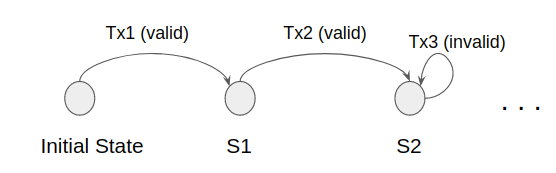
\includegraphics[width=0.6\textwidth,keepaspectratio]{figures/utxo_growth/state_machine.png}
    \caption{A decentralized state machine model for a distributed ledger.}
    \label{fig:state-machine}
\end{figure}

Our formalism is similar to chimeric ledgers~\cite{chimeric}, though focused on
UTxO-based ledgers. Following, we provide some basic definitions in a
``top-down'' approach, starting with the ledger $\ledger$, which is an ordered
list of transactions; our notation of functions is the one typically
used in functional programming languages, for example a function $f : A
\rightarrow B
\rightarrow C$ takes two input parameters of type $A$ and $B$ respectively and
returns a value of type $C$.

\begin{definition}
    A \emph{ledger} $\ledger$ is a list of valid transactions: $\ledger \defn \mathit{List}[\mathit{Transaction}]$.
\end{definition}

A transaction $\tx$ transitions the system from one state to another.
UTxO-based transactions are thus a product of \emph{inputs}, which define the
ownership of assets, and \emph{outputs}, which define the rules of
re-transferring the acquired value.

\begin{definition}
    A UTxO-based transaction $\tx$ is :
    $\mathit{Transaction} \defn (\mathit{inputs}: \mathit{Set}[\mathit{Input}],
                       \mathit{outputs}: \mathit{List}[\mathit{UTxO}],
                       \mathit{forge}: \mathit{Value},
                       \mathit{fee}: \mathit{Value})$
\end{definition}

An \emph{unspent transaction output (UTxO)} represents the ownership of some
value from a party, which is represented via an \emph{address} $\addr$.
Intuitively, in the real world, an output is akin to owning a physical coin of
an arbitrary denomination.

\begin{definition}\label{def:utxo}
    A UTxO is defined as follows: $\mathit{UTxO} \defn (\addr: \mathit{Address},\ \mathit{value}: \mathit{Value},\ \mathit{created}: \mathit{Timestamp})$.
\end{definition}

A transaction's input is a reference to a UTxO, \ie an output that is owned by
the party that creates the transaction. An input consists of two objects:
\begin{inparaenum}[i)]
    \item the \emph{id} of the transaction that created it (typically its hash)
        and
    \item an index, which identifies the specific output among all UTxOs of the
        referenced transaction.
\end{inparaenum}

\begin{definition}
    An input is defined as: $\mathit{Input} \defn (\mathit{id}: \mathit{Hash}, \mathit{index}: \mathit{Int})$.
\end{definition}

Given an input and a ledger, three functions retrieve:
\begin{inparaenum}[i)]
    \item the corresponding output,
    \item the corresponding transaction, and
    \item the input value.
\end{inparaenum}
All returned values are wrapped in \verb|Option|, denoting that a value may not
be returned.

\begin{itemize}
    \item $\utxo: \inp \rightarrow \ledger \rightarrow \verb|Option|[\utxo]$
    \item $\tx: \inp \rightarrow \ledger \rightarrow
        \verb|Option|[\mathit{Transaction}]$
    \item $\mathit{value}: \inp \rightarrow \ledger \rightarrow \verb|Option|[\mathit{Value}]$
\end{itemize}

A transaction defines some value that is given as a \emph{fee} to the
\emph{miner}, \ie the party who publishes the transaction into the ledger
$\ledger$. We require that all transactions must preserve value as
follows:
$\tx.\mathit{forged} + \sum_{i \in \tx.\mathit{inputs}}^{} \mathit{value}(i, \ledger) = \tx.\mathit{fee} + \sum_{o \in \tx.\mathit{outputs}}^{} o.\mathit{value}$.
We note that this applies only on standard transactions, not ``coinbase''
transactions which create new coins.

Finally, we define the ledger's state $\ledgerState$. $\ledgerState$ comprises
the \emph{UTxO set}, \ie the set of all outputs of transactions whose value
has not been re-transferred and can be used as inputs to new transactions.

\begin{definition}\label{def:lstate}
    The ledger's state is defined as: $\mathit{State} \defn \mathit{Set}[\mathit{Input}]$.
\end{definition}

We now return to the state machine model. A transaction is applied on a ledger
state $\ledgerState_1$ and results in a ledger state $\ledgerState_2$ via the
function:
\begin{align*}
    \mathsf{txRun}: \mathit{Transaction} \rightarrow \mathit{LedgerState} \rightarrow \mathit{LedgerState}
\end{align*}
An ordered list of transactions $\txSet = [\tx_1, \tx_2, \dots, \tx_N]$ can be
applied sequentially on state $\ledgerState_1$ to transit to state
$\ledgerState_N$: $\ledgerState_N = (\mathsf{txRun}(\tx_N).\; \dots\;
.\mathsf{txRun}(\tx_2) .  \mathsf{txRun}(\tx_1))(\ledgerState_1)$, assuming the
function composition operator (.).

Finally, every ledger state $\ledgerState$ corresponds to some cost
$\stateCost$.  We assume a cost function, which assigns a signed integer of
cost units to a ledger state.
\begin{align*}
    \mathsf{cost}: \mathit{LedgerState} \rightarrow \mathit{Cost}
\end{align*}
This function is employed in
Definition~\ref{def:tx-cost}, which defines a transaction's cost; minimizing
this cost will be the target of our optimization. Observe that the
transaction's cost might be negative, \eg if the transaction reduces the state.

\begin{definition}\label{def:tx-cost}
    The cost of a transaction $\tx$ applied to a state $\ledgerState$ is the
    difference between the cost of the final state minus the cost of the
    initial state:

    \begin{math}\\
        \mathsf{costTx}: \mathit{Transaction} \rightarrow \mathit{LedgerState} \rightarrow \mathit{Cost} \\
        \mathsf{costTx}(\tx, \ledgerState) = cost(\mathsf{txRun}(\tx,
        \ledgerState)) - \mathit{cost}(\ledgerState)\\
    \end{math}

        The cost of an ordered list of transactions $[T]$ applied to a state
        $\ledgerState$ is the difference between the cost of the final state
        minus the cost of the initial state:

	\begin{math}\\
            \mathsf{costTotTx}: [\mathit{Transaction}] \rightarrow \mathit{LedgerState} \rightarrow
                \mathit{Cost}\\
		\mathsf{costTotTx}([T], \ledgerState) =
                        \mathit{cost}((\mathsf{txRun}(\tx_N).\; \dots\; .\mathsf{txRun}(\tx_2) .
                        \mathsf{txRun}(\tx_1))(\ledgerState_1)) - \mathit{cost}(\ledgerState)
	\end{math}
\end{definition}

We note that cost represents the size of the ledger's state. However, our model
is generic enough to accommodate alternative cost designs as well. For
instance, cost could represent the computational effort of producing or
verifying the state, such that a cost unit would be a computational cycle.
Therefore, our analysis would also be directly applicable in that case, by
accordingly adapting some parts of the subsequent optimization framework like
the heuristics.
